%\setchapterimage{bandeau}
\chapter*{TD \arabic{cptTD} \\ 
Système de freinage d'un TGV DUPLEX -- 
\ifprof Corrigé \else Sujet \fi}
\addcontentsline{toc}{section}{TD \arabic{cptTD} :
Système de freinage d'un TGV DUPLEX -- 
\ifprof Corrigé \else Sujet \fi}

\iflivret \stepcounter{cptTD} \else
\ifprof  \stepcounter{cptTD} \else \fi
\fi

\setcounter{question}{0}
\marginnote{Centrale Supelec -- PSI -- 2006.}
\marginnote[1cm]{
\UPSTIcompetence[2]{C1-02}
\UPSTIcompetence[2]{C2-04}}

\begin{marginfigure}[4cm]
\centering
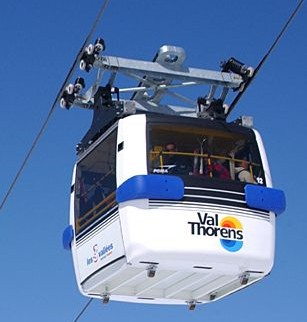
\includegraphics[width=\linewidth]{fig_00}
\end{marginfigure}

\subsection*{Présentation}

Par sécurité, il est nécessaire que la distance d'arrêt d'une rame de t TGV soit inférieure à \SI{2500}{m}. 

Lors du freinage il est indispensable que les roues du train ne se bloquent pas. Le phénomène de blocage appelé enrayage 
a pour effet de déformer les roues et les rails et peut entraîner le déraillement du train. 

\subsection*{Dispositif d'anti-enrayage}
L’objectif de cette partie est l’étude de la loi de commande du dispositif d’anti-enrayage
et plus précisément le calcul du correcteur de la boucle de régulation en
vue de satisfaire un cahier des charges qui sera exprimé par la suite.

Le glissement relatif entre la roue et le rail est noté $\nu$ et peut s'exprimer sous la forme $\nu=1-\dfrac{V_R}{V_T}$ où $V_T$ est la vitesse de translation du train par rapport aux rails et $V_R$ l'opposée de la vitesse du point de contact appartenant à la roue par rapport à son support (bogie).
%
%La réalisation de la régulation de glissement ne peut être effectuée directement,
%en particulier la seule mesure généralement disponible est celle de la vitesse $V_R$, aussi la vitesse $V_T$ est obtenue par estimation. En « pratique », la mise en
%place de la chaîne de régulation du dispositif d’anti-enrayage du système de freinage
%est conçue de la façon suivante :
%\begin{itemize}
%\item elle est réalisée au travers de l’asservissement des vitesses des roues à une
%consigne de référence obtenue à partir de $V_T$;
%\item la commande de l’actionneur est non linéaire, de type tout ou rien ;
%\item les algorithmes implémentés visent à optimiser le point de fonctionnement
%en vue de minimiser la distance de freinage.
%\end{itemize}

Dans le cadre de cette étude, on supposera que :
\begin{itemize}
\item les vitesses $V_R$ et $V_T$ sont directement accessibles à la mesure, éventuellement
entachées d’une erreur;
\item la régulation peut se ramener directement à celle du glissement;
\item  le comportement de l’actionneur et de sa « commande rapprochée » est modélisé
par une fonction de transfert linéaire correspondant à un comportement
« moyen ».
\end{itemize}
On suppose, pour la suite, que l’architecture de la boucle de régulation est représentée sur la figure suivante où est la consigne de glissement.

\begin{marginfigure}
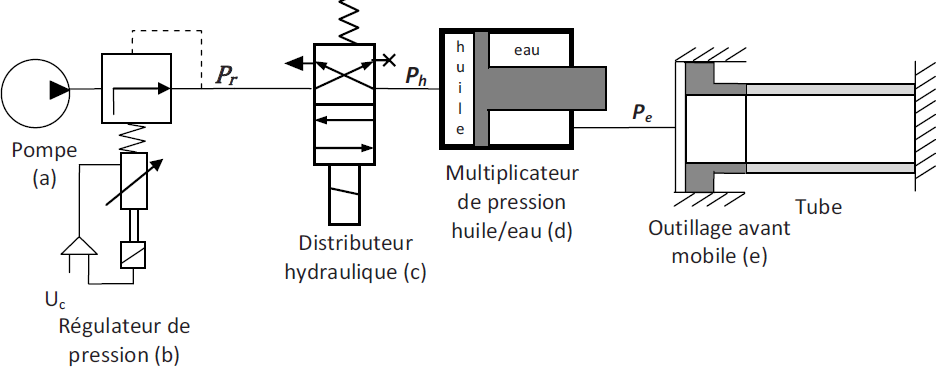
\includegraphics[width=\linewidth]{fig_01}
%%\textit{}
\end{marginfigure}


\begin{itemize}
\item $H_1(p)$ : fonction de transfert de l’actionneur de freinage (vérin pneumatique
+ électro-valve);
\item $H_2(p)$ : fonction de transfert de la roue au freinage;
\item $C(p)$ : correcteur de la boucle de régulation;
\item $M(p)$ : fonction de transfert de la chaîne de mesure du glissement obtenu à
partir des vitesses $V_T$ et $V_R$, cette chaîne comporte un filtre destiné à limiter
l’impact des bruits de mesure;
\item $\nu_m$ : glissement estimé à partir de $V_T$ et de $V_R$.
\end{itemize}

On adoptera pour la suite : $H_1(p)=\dfrac{2000}{1+0,1p+0,01p^2}$,  $H_2(p)=\dfrac{K_h}{p} = \dfrac{45\cdot 10^{-6}}{p}$ et $M(p)=\dfrac{1}{1+0,05 p}$.

Pour une vitesse $V_T=\SI{200}{km.h^{-1}}$, le cahier des charges est résumé par les données 
du tableau suivant et les données numériques utilisées sont données ci-dessous.
Enfin, les problèmes liés à l’évolution de la vitesse $V_T$ ne font pas l’objet de cette
étude.


\begin{marginfigure}
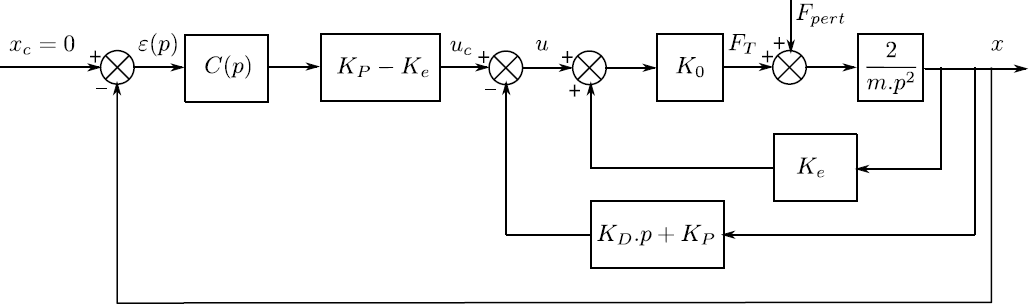
\includegraphics[width=\linewidth]{fig_02}
%%\textit{}
\end{marginfigure}

%On note $M=\SI{8200}{kg}$, $V_T=\SI{200}{km.h^{-1}}$, $\dfrac{I}{r^2}=\SI{400}{kg}$, $g=\SI{10}{m.s^{-2}}$.

\subsection*{Analyse des réponses fréquentielles en boucle ouverte}

%On donne $H_2(p)=\dfrac{r^2/\left( IV_{T0}\right)}{p} = \dfrac{45\cdot 10^{-6}}{p}$.

\subparagraph{}
\textit{En prenant $C(p)=1$, compléter par le tracé asymptotique le diagramme
de Bode de la fonction de transfert en boucle ouverte fourni en figure suivante
en justifiant le tracé.}

\begin{marginfigure}
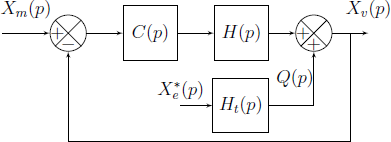
\includegraphics[width=\linewidth]{fig_03}
%\textit{}
\end{marginfigure}

\subsection*{Synthèse du régulateur de la boucle de régulation}
On décide d’implémenter un régulateur de type P.I. dont la fonction de transfert
est : $C(p)=K_R\left( 1+\dfrac{1}{T_i p}\right)$.

\question{Donner l'allure du diagramme de Bode de ce correcteur.}
\question{Calculer la valeur que doit prendre l’argument de $C(p)$ afin d’assurer
la marge de phase imposée par le cahier des charges à la pulsation de coupure $\omega_c$
souhaitée.}

\question{Calculer la valeur minimale $T_{i\text{min}}$ , que l’on peut conférer à la constante $T_i$ de l’action intégrale du régulateur.}


\question{En adoptant $T_i=T_{i\text{min}}$, déterminer alors le gain $K_r$ du régulateur permettant de satisfaire la pulsation de coupure et la marge de phase souhaitées.
}


\question{Le système étant bouclé par le régulateur dimensionné à la question
précédente, déterminer la marge de gain (avec très peu de calcul). Conclure sur les marges de stabilité obtenues.}

\subsection*{Vérification du cahier des charges vis-à-vis de la consigne de glissement}

Le correcteur de la boucle de régulation du dispositif d’anti-enrayage a été déterminé
à partir de considérations sur la réponse fréquentielle en boucle ouverte
(pulsation de coupure à  $\SI{0}{dB}$ et marge de phase). Aussi l’objectif de cette partie
est de vérifier que le correcteur déterminé permet de satisfaire le cahier des charges.
Cette vérification concerne d’une part les performances vis-à-vis des variations
de la consigne de glissement : temps du 1\ier maximum, dépassement, écart
en régime permanent et d’autre part la réponse vis-à-vis des variations d’adhérence.

Au regard de la réponse fréquentielle en boucle fermée $F(p)=\dfrac{\nu_1(p)}{\nu_c(p)}$, on décide de modéliser la transmittance correspondante par la fonction suivante : 
$$
F(p)=\dfrac{\nu_1(p)}{\nu_c(p)} = \dfrac{K_f\left(1+\tau_1 p\right)}{\left(1+\tau_2 p\right)^2 \left( 1+\dfrac{2\xi}{\omega_0}p + \dfrac{p^2}{\omega_0^2} \right)}.
$$

On suppose sans aucune justification que $\omega_0> \dfrac{1}{\tau_2}$. 

\question{En examinant les diagrammes de Bode fournis sur la figure suivante de la fonction de
transfert en boucle fermée $F(p)=\dfrac{\nu_1(p)}{\nu_c(p)}$, justifier l’expression adoptée et
compléter les diagrammes fournis par leur tracé asymptotique.}

\begin{marginfigure}
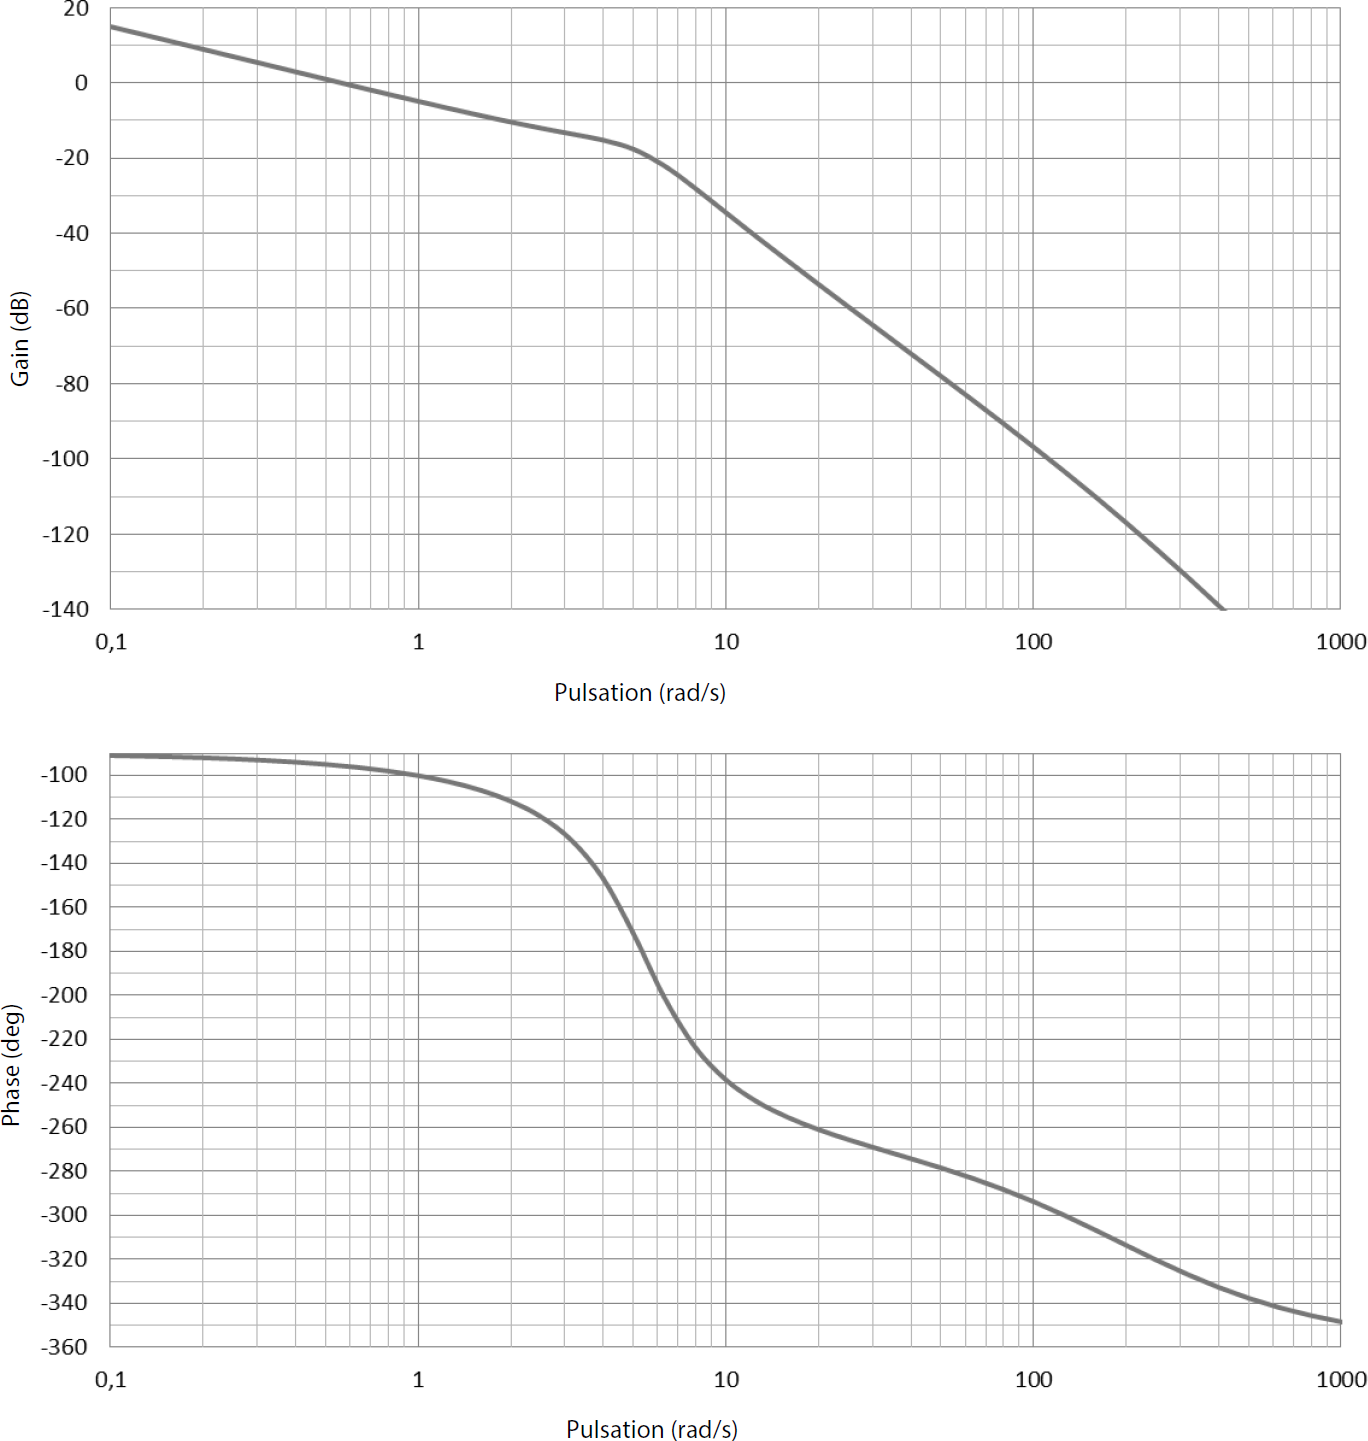
\includegraphics[width=\linewidth]{fig_04}
%\textit{}
\end{marginfigure}


\question{Proposer les valeurs numériques pour les différents paramètres associés à
cette fonction de transfert.}

\question{En justifiant, montrer que l’on peut approcher la fonction de
transfert par la forme suivante : $F(p)=\dfrac{K_f \left(1
+\tau_1 p \right)}{\left(1
+\tau_2 p \right)^2}$.}

\begin{obj}
Calcul de la réponse temporelle vis-à-vis de la consigne de glissement. 
\end{obj}

\question{En utilisant la relation ci-dessous, montrer que l’évolution temporelle de
la réponse impulsionnelle $f(t)$ du système décrit par la fonction de transfert $F(p)$, peut être exprimée par la relation suivante où $y(t)$ est une fonction que vous préciserez, $a$ et $b$ deux constantes que vous exprimerez en fonction de $K_f$, $\tau_1$ et $\tau_2$ : $f(t)=ay(t)+b\dot{y}(t)$. On donne $\mathcal{L}\left[ t^n e^{-at} h(t)\right]=\dfrac{n!}{\left(p+a\right)^{n+1}}$ ($h(t)$ fonction de heaviside -- échelon unité).}

\question{À partir de cette réponse, calculer le temps du 1\ier maximum et en déduire le
dépassement en réponse à une variation en échelon de la consigne de glissement
relatif $\nu_c(t)=\nu_{c0}h(t)$.}

\question{Vérifier le cahier des charges en réponse à une variation en échelon de la consigne
de glissement relatif.}

\subsection*{Analyse des performances temporelles en réponse à des variations d’adhérence}

La variation d’adhérence peut être modélisée en première approximation comme une force perturbatrice externe additive $f_{\text{ext}}$. On admet que cette modélisation conduit au schéma-blocs représenté sur la figure ci-dessous.


\begin{marginfigure}
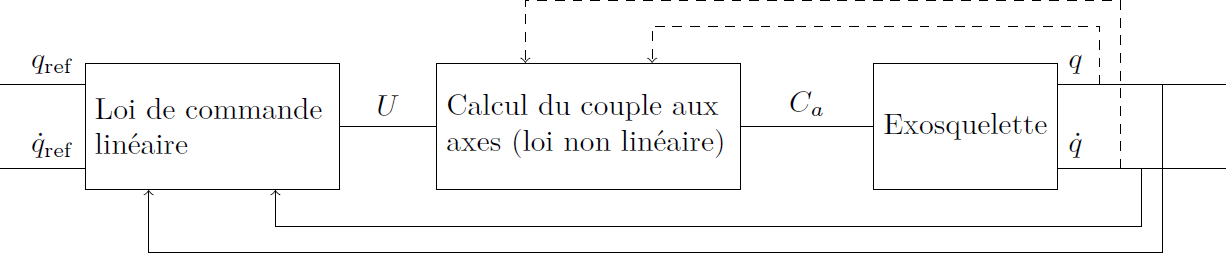
\includegraphics[width=\linewidth]{fig_07}
%\textit{}
\end{marginfigure}


On se propose dans cette partie d’évaluer les performances de la chaîne de régulation de freinage vis-à-vis de cette perturbation.

\question{Déterminer la fonction de transfert $F_2(p)=\dfrac{\nu_1(p)}{F_{\text{ext}}(p)}$ entre le glissement et la force de perturbation que vous expliciterez en fonction des différentes
transmittances de la boucle de régulation (On rappelle qu'en régulation on considère l'entrée principale égale à 0). En expliquant soigneusement
votre démarche, montrer que le module de la réponse fréquentielle, notée $\left|\left| F_2\left(j\omega\right) \right|\right| $ , de cette fonction peut être approché par la relation : }
$$
||F_2 \left(j \omega\right) || = 
\min \left(
||H_2\left(j \omega\right)||; 
\left|\left| \dfrac{1}{C\left(j \omega\right)H_1\left(j \omega\right)M\left(j \omega\right)}\right|\right|\right).
$$


\begin{obj}
Calcul de la fonction de transfert $F_2(p)$.
\end{obj}
On donne le tracé de la fonction $\left|\left| \dfrac{1}{C\left(j \omega\right)H_1\left(j \omega\right)M\left(j \omega\right)}\right|\right|$. 

\begin{marginfigure}
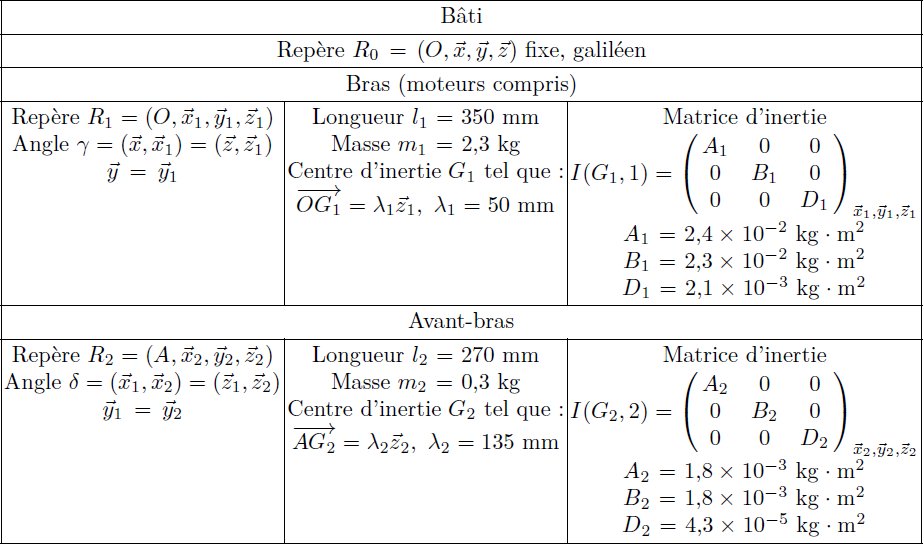
\includegraphics[width=\linewidth]{fig_06}
%\textit{}
\end{marginfigure}

\question{Tracer le diagramme asymptotique de $\left|\left| H_2 \left(  j\omega \right)\right|\right|$.}

\question{En déduire la forme du tracé asymptotique de la fonction $\left|\left| F_2 \left(  j\omega \right)\right|\right|$. En analysant
les brisures de ce diagramme et en supposant que le système bouclé est
stable, donner directement sous forme numérique, l’expression de la fonction de
transfert $F_2(p)=\dfrac{\nu_1(p)}{F_{\text{ext}}(p)}$ entre le glissement et la perturbation due à la
variation d’adhérence.}

\begin{obj}
Calcul de l’évolution du glissement en réponse à une variation de l’adhérence.
\end{obj}

\question{Préciser les pôles de la fonction $F_2(p)$ déterminée à la question précédente et en
justifiant votre réponse proposer une fonction approchée de cette fonction sous
la forme $F_2(p)=\dfrac{K_2 p}{1+Tp}$.}

\question{En utilisant cette fonction de transfert, donner l’expression de l’évolution
temporelle du glissement relatif $\nu_1(p)$ en réponse à une variation en échelon de
la force perturbatrice $F_{\text{ext}}=F_0 h(t)$ avec $F_0=\SI{2000}{N}$.}

\question{Tracer l’allure de l’évolution temporelle du glissement relatif $\nu_1(p)$ en précisant
la valeur initiale $\nu_1(0)$. En vous référant à des fonctions ou des résultats
connus, déterminer un ordre de grandeur du temps de réponse $t_r$ à partir
duquel le glissement reste en dessous de 5\,\% de la valeur initiale (valeurs
à considérer en valeur absolue).}

\question{Conclure sur les performances obtenues vis-à-vis des exigences du cahier des
charges en réponse à des variations de l’adhérence.}


\begin{solution}
\begin{multicols}{2}
\begin{enumerate}
\item $\quad$.
\item $\quad$.
\item $-20\degres$.
\item $T_i\geq 2,75$.
\item $K=11$.
\item $MG = \SI{18}{dB}$ et $M \varphi  = 60\degres$.
\item $\quad$.
\item $K_f=1$, $\tau_1=1/0,3$, $\tau_2=1/0,6$, $\omega_0=\SI{10}{rad.s^{-1}}$, $\xi<0,7$.
\item $\dfrac{1+3,3 p}{\left(1+1,66 p\right)^2}$.
\item $f(t)=\left( \dfrac{\tau_2-\tau_1}{\tau_2^3}t+\dfrac{\tau_1}{\tau_2^2}\right) e^{-t/\tau_2}h(t)$.
\item $t_m=\dfrac{\tau_2\tau_1}{\tau_1-\tau_2}=\SI{3,3}{s}$ et dépassement de 13\%.
\item $\quad$.
\item $\quad$.
\item $\quad$.
\item $F_2(p)=-\dfrac{\dfrac{p}{12100}}{\left(1+2,8p\right)\left(1+0,5p\right)}$.
\item $p_1=-0,35$ et $p_2=-2$. $F_2(p)=-\dfrac{\dfrac{p}{12100}}{\left(1+2,8p\right)}$.
\item $\nu_1(t)=-\dfrac{K_2}{T}F_0 e^{-t/T}h(t)$.
\end{enumerate} 
\end{multicols}
\end{solution}
 